\subsection{原理と方法}

\paragraph{原理}
各観測 $i=1,\dots,N$ で $y_i\in\mathbb{R}^m$, $X_i\in\mathbb{R}^{m\times p}$ とし
\[
y_i = X_i\theta + w_i,\qquad \mathbb{E}[w_i]=0,\ \mathrm{Cov}(w_i)=V\ (\text{既知}), 
\]
を仮定する。$Q:=V^{-1}$ とおく。WLS は重み付き残差平方和
\[
J(\theta)=\sum_{i=1}^N (y_i-X_i\theta)^\top Q\,(y_i-X_i\theta)
\]
を最小化する推定で,正規方程式は
\[
S\hat\theta=b,\qquad 
S:=\sum_{i=1}^N X_i^\top QX_i,\quad 
b:=\sum_{i=1}^N X_i^\top Qy_i.
\]
したがって
\[
\hat\theta=(\sum_{i=1}^N X_i^\top QX_i)^{-1}\Big(\sum_{i=1}^N X_i^\top Qy_i\Big).
\]
$V$ が既知のとき
\[
\mathrm{Cov}(\hat\theta)=S^{-1}.
\]
$V=\sigma^2\Sigma$ のようにスケール未知なら
\[
\hat\sigma^2=\frac{\sum_{i=1}^N r_i^\top \Sigma^{-1} r_i}{Nm-p},\quad r_i:=y_i-X_i\hat\theta,\qquad
\widehat{\mathrm{Cov}}(\hat\theta)=\hat\sigma^2\,(\sum X_i^\top \Sigma^{-1}X_i)^{-1}.
\]

\paragraph{方法}
(1) 各 $i$ の設計行列 $X_i$ と観測 $y_i$ を用意($X_i$ は $m\times p$)。  
(2) $Q=V^{-1}$ を決めて $S=\sum X_i^\top QX_i,\ b=\sum X_i^\top Qy_i$ を計算。  
(3) $\hat\theta=S^{-1}b$。  

\paragraph{実装}
R による実装例を以下に示す。
\begin{lstlisting}
regression_multiple <- function(x, y, V = NULL, Q = NULL){
    # y: n×1行列(またはベクトル)
    if (is.null(ncol(y))) {
        y <- as.matrix(y, ncol = 1)
    }
    if (length(dim(x)) != 3) {
        stop("x must be a 3-dimensional array")
    }
    n <- dim(x)[3]
    m <- ncol(y)
    p <- dim(x)[1] # 特徴量数
    S <- matrix(0, p, p)
    b <- matrix(0, p, 1)
    T <- matrix(0, p, p)
    if (is.null(V)) {
        V <- diag(m)
    }
    if (is.null(Q)) {
        Q <- solve(V)
    }
    # m=1(スカラー出力)の場合はQ,Vをスカラー化
    if (m == 1) {
        Q <- as.numeric(Q)
        V <- as.numeric(V)
        for (i in 1:n) {
            xi <- as.matrix(x[,,i]) # (p,1)
            S <- S + xi %*% t(xi) * Q
            b <- b + xi * Q * y[i, 1]
            T <- T + xi %*% t(xi) * V
        }
    } else {
        for (i in 1:n) {
            xi <- as.matrix(x[,,i])
            yi <- matrix(y[i, ], nrow = m, ncol = 1)
            S <- S + t(xi) %*% Q %*% xi
            b <- b + t(xi) %*% Q %*% yi
            T <- T + t(xi) %*% V %*% xi
        }
    }
    theta_hat <- solve(S) %*% b
    err_cov_mat <- solve(S) %*% T %*% solve(S)
    return(list(theta_hat = theta_hat, err_cov_mat = err_cov_mat, S = S, b = b, T = T))
}
\end{lstlisting}

\subsection{課題5(2次元出力:重み付き最小二乗法)}

\paragraph{課題の内容}
入力 $x_i \in \mathbb{R}$($i=1,\dots,1000$)に対し,$m=2$ 次元出力の線形モデル
\[
  y_i \;=\; \phi(x_i)\,\theta \;+\; w_i,\qquad
  \phi(x) = 
  \begin{bmatrix}
    1 & x\\
    1 & x^2
  \end{bmatrix},
  \quad
  w_i \sim \mathcal{N}(0,V),\;
  V=\begin{bmatrix}100&0\\0&1\end{bmatrix},
\]
を考える.ここで $\theta\in\mathbb{R}^2$ を推定対象とする.

\paragraph{推定法}
最小二乗(OLS)の推定値は
\[
  \hat{\theta}_N \;=\;
  \Bigl(\sum_{i=1}^N \phi_i^\top \phi_i \Bigr)^{-1}
  \sum_{i=1}^N \phi_i^\top y_i,
\]
で与えられる($\phi_i=\phi(x_i)$).
観測雑音の共分散 $V$ が既知で,その影響を反映した重み付き最小二乗(WLS)を用いると,
$V=W^2$ を満たす $W$ に対し
\[
  \hat{\theta}_N \;=\;
  \Bigl(\sum_{i=1}^N \phi_i^\top W^{-2}\phi_i \Bigr)^{-1}
  \sum_{i=1}^N \phi_i^\top W^{-2} y_i
  \;=\;
  \Bigl(\sum_{i=1}^N \phi_i^\top Q\,\phi_i \Bigr)^{-1}
  \sum_{i=1}^N \phi_i^\top Q\, y_i,
\]
となる($Q=W^{-2}=V^{-1}$).

\paragraph{実装}
\texttt{datas/mmse\_kadai5.csv} を読み込み,$x$ から
\(
\phi(x)=\begin{bmatrix}1&x\\1&x^2\end{bmatrix}
\)
を構成して $x\in\mathbb{R}^{2\times 2\times N}$ の 3 次元配列とし,
$y\in\mathbb{R}^{N\times 2}$ を観測行列とした.
推定は関数 \texttt{regression\_multiple} を用い,
\textbf{OLS} は無重み($Q=I$),
\textbf{WLS} は $V=\mathrm{diag}(100,1)$ を渡し内部で $Q=V^{-1}$ を用いる設定とした.
また,$N\in\{4,8,16,32,64,128,256,512,1000\}$ に対する
$\hat{\theta}_N$ の収束の様子を片対数($x$ 軸のみ対数)で可視化した.

\paragraph{結果}
全データ($N=1000$)を用いた推定結果は次のとおりである.

\medskip
\noindent\textbf{OLS}
\[
  \hat{\theta}_{\mathrm{OLS}}=
  \begin{bmatrix}
    2.994567\\[-1mm]
   -2.068971
  \end{bmatrix},\qquad
  \widehat{\mathrm{Cov}}(\hat{\theta}_{\mathrm{OLS}})=
  \begin{bmatrix}
    5.7621\!\times\!10^{-4} & -1.5041\!\times\!10^{-4}\\
    -1.5041\!\times\!10^{-4} & 2.9684\!\times\!10^{-4}
  \end{bmatrix}.
\]

\noindent\textbf{WLS}
\[
  \hat{\theta}_{\mathrm{WLS}}=
  \begin{bmatrix}
    2.939084\\[-1mm]
   -1.986465
  \end{bmatrix},\qquad
  \widehat{\mathrm{Cov}}(\hat{\theta}_{\mathrm{WLS}})=
  \begin{bmatrix}
    2.39993\!\times\!10^{-1} & -9.66541\!\times\!10^{-2}\\
    -9.66541\!\times\!10^{-2} & 4.99126\!\times\!10^{-2}
  \end{bmatrix}.
\]

\begin{figure}[H]
  \centering
  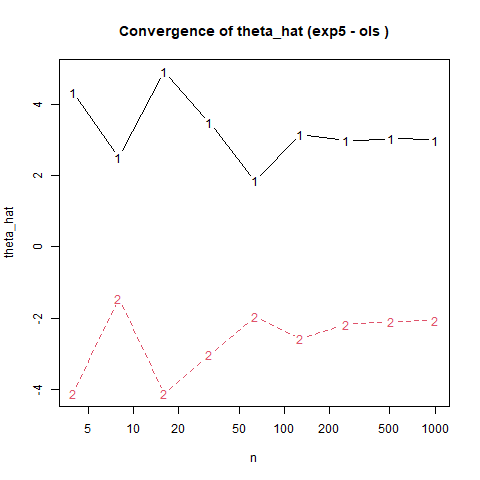
\includegraphics[width=.82\linewidth]{graphs/task5_ols.png}
  \caption{$\hat{\theta}_N$ の収束(OLS)}
  \label{fig:task5_ols}
\end{figure}

\begin{figure}[H]
  \centering
  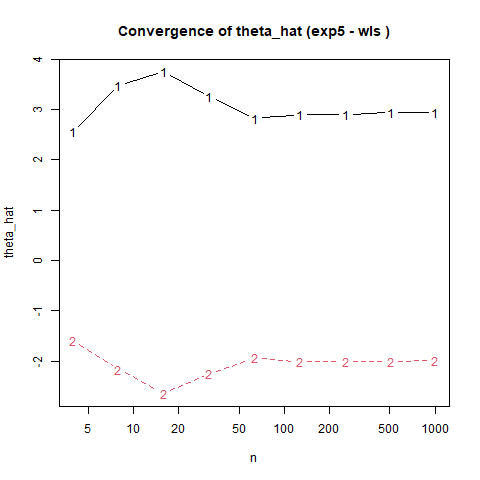
\includegraphics[width=.82\linewidth]{graphs/task5_wls.png}
  \caption{$\hat{\theta}_N$ の収束(WLS,$V=\mathrm{diag}(100,1)$)}
  \label{fig:task5_wls}
\end{figure}

\paragraph{考察}
% (ここに考察を記述)


\subsection{課題6(2次元出力・異分散2群に対する重み付き最小二乗)}

\paragraph{課題の内容}
入力 $x_i\in\mathbb{R}$ に対し,
\[
  y_i \;=\; \phi(x_i)\,\theta + w_i,\qquad
  \phi(x)=
  \begin{bmatrix}
    1 & x\\[1mm]
    1 & x^2
  \end{bmatrix},\quad
  \theta\in\mathbb{R}^2,
\]
という $m=2$ 次元出力の線形モデルを考える.雑音は $N$ サンプルのうち前半 $i=1,\dots,\texttt{num}$ が
$w_i\sim\mathcal{N}(0,V_1)$,後半 $i=\texttt{num}+1,\dots,N$ が $w_i\sim\mathcal{N}(0,V_2)$ に従うとする.
本課題では $V_1=\mathrm{diag}(100,1)$,$V_2=\mathrm{diag}(2,1)$,$\texttt{num}=500$ を既知として推定を行う.

\paragraph{推定法(GLS/WLS)}
$Q_k=V_k^{-1}$($k=1,2$)とおくと,一般化最小二乗(WLS)の正規方程式は
\[
  S\,\hat{\theta}_N \;=\; b,
  \quad
  S \;=\; \sum_{i=1}^{\texttt{num}}\!\phi_i^\top Q_1\phi_i \;+\; \sum_{i=\texttt{num}+1}^{N}\!\phi_i^\top Q_2\phi_i,
  \quad
  b \;=\; \sum_{i=1}^{\texttt{num}}\!\phi_i^\top Q_1 y_i \;+\; \sum_{i=\texttt{num}+1}^{N}\!\phi_i^\top Q_2 y_i,
\]
より
\[
  \hat{\theta}_N \;=\; S^{-1} b.
\]
標本ベースの誤差共分散推定は(実装に合わせて)
\[
  \widehat{\mathrm{Cov}}(\hat{\theta}_N)
  \;=\;
  S^{-1}\,T\,S^{-1},\qquad
  T \;=\; \sum_{i=1}^{\texttt{num}}\!\phi_i^\top V_1\phi_i \;+\; \sum_{i=\texttt{num}+1}^{N}\!\phi_i^\top V_2\phi_i .
\]
なお OLS は $Q_1=Q_2=I$ とした特別な場合である.

\paragraph{実装}
\texttt{datas/mmse\_kadai6.csv} から $x$ を読み,$\phi(x)$ を用いて
$x\in\mathbb{R}^{2\times2\times N}$,$y\in\mathbb{R}^{N\times2}$ を構成した.
推定は関数 \texttt{regression\_multiple\_different\_distributions} により,
前半 $V_1$,後半 $V_2$ の重みで $S,b,T$ を分割加算して $\hat{\theta}_N$ と
$\widehat{\mathrm{Cov}}(\hat{\theta}_N)$ を得た.
また $N$ を \texttt{ns = seq(4,1000,length.out=20)} で走らせ,
$\hat{\theta}_N$ の収束の様子を折れ線で可視化した($x$ 軸は線形目盛).

\paragraph{結果}
全データ($N=1000$,$\texttt{num}=500$)の推定結果は以下のとおりである.

\medskip
\noindent\textbf{OLS(比較)}
\[
  \hat{\theta}_{\mathrm{OLS}}=
  \begin{bmatrix}
    3.188356\\[-1mm]
   -2.092183
  \end{bmatrix},\qquad
  \widehat{\mathrm{Cov}}(\hat{\theta}_{\mathrm{OLS}})=
  \begin{bmatrix}
    5.692084\!\times\!10^{-4} & -1.402629\!\times\!10^{-4}\\
    -1.402629\!\times\!10^{-4} & 2.842674\!\times\!10^{-4}
  \end{bmatrix}.
\]

\noindent\textbf{WLS($V_1=\mathrm{diag}(100,1)$,$V_2=\mathrm{diag}(2,1)$)}
\[
  \hat{\theta}_{\mathrm{WLS}}=
  \begin{bmatrix}
    2.994202\\[-1mm]
   -2.014699
  \end{bmatrix},\qquad
  \widehat{\mathrm{Cov}}(\hat{\theta}_{\mathrm{WLS}})=
  \begin{bmatrix}
    6.019710\!\times\!10^{-2} & -2.227335\!\times\!10^{-2}\\
    -2.227335\!\times\!10^{-2} & 1.276759\!\times\!10^{-2}
  \end{bmatrix}.
\]

\begin{figure}[H]
  \centering
  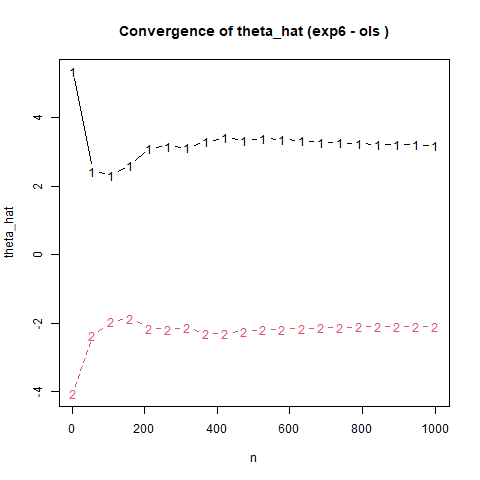
\includegraphics[width=.82\linewidth]{graphs/task6_ols.png}
  \caption{$\hat{\theta}_N$ の収束(OLS)}
  \label{fig:task6_ols}
\end{figure}

\begin{figure}[H]
  \centering
  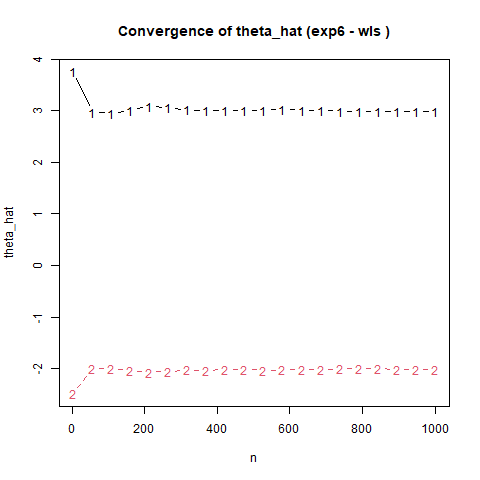
\includegraphics[width=.82\linewidth]{graphs/task6_wls.png}
  \caption{$\hat{\theta}_N$ の収束(WLS,$V_1$/$V_2$ 異分散)}
  \label{fig:task6_wls}
\end{figure}

\paragraph{考察}
% (ここに考察を記述)
